\documentclass[aspectratio=169]{beamer}

\usetheme{Boadilla}
\usefonttheme{professionalfonts}
\setbeamertemplate{navigation symbols}{}
\setbeamertemplate{itemize items}[circle]
\setbeamertemplate{enumerate items}[default]
\setbeamertemplate{headline}{}

\usepackage[utf8]{inputenc}
\usepackage[T1]{fontenc}
\usepackage{lmodern}
\usepackage{amsmath}
\usepackage{booktabs}
\usepackage{tabularx}
\usepackage{array}
\usepackage{hyperref}
\usepackage[strings]{underscore}
\usepackage{listings}
\usepackage{tikz}
\usetikzlibrary{arrows.meta,positioning,fit,calc,shapes.geometric}
\usepackage{xcolor}

\definecolor{courseblue}{HTML}{12355B}
\definecolor{coursegold}{HTML}{C98A2E}
\definecolor{courseice}{HTML}{EEF3F8}
\definecolor{coursegreen}{HTML}{2F6B4F}
\definecolor{coursegray}{HTML}{4B5563}
\definecolor{codebg}{HTML}{F7F9FC}
\definecolor{codecomment}{HTML}{5E6C84}
\definecolor{codestring}{HTML}{0B6E4F}

\setbeamercolor{palette primary}{bg=courseblue,fg=white}
\setbeamercolor{palette secondary}{bg=coursegold,fg=white}
\setbeamercolor{palette tertiary}{bg=courseblue,fg=white}
\setbeamercolor{palette quaternary}{bg=coursegold,fg=white}
\setbeamercolor{structure}{fg=courseblue}
\setbeamercolor{frametitle}{bg=courseice,fg=courseblue}
\setbeamercolor{title}{fg=courseblue}
\setbeamercolor{block title}{bg=courseblue,fg=white}
\setbeamercolor{block body}{bg=courseice,fg=black}
\setbeamercolor{normal text}{fg=black,bg=white}
\setbeamercolor{alerted text}{fg=coursegold}

\setbeamerfont{footline}{size=\scriptsize}

\setbeamertemplate{footline}{
  \leavevmode
  \hbox{
    \begin{beamercolorbox}[wd=.33\paperwidth,ht=2.8ex,dp=1.2ex,leftskip=0.8em]{palette primary}%
      University of Trieste
    \end{beamercolorbox}%
    \begin{beamercolorbox}[wd=.49\paperwidth,ht=2.8ex,dp=1.2ex,center]{palette tertiary}%
      \coursename{} \textbar{} \coursecode
    \end{beamercolorbox}%
    \begin{beamercolorbox}[wd=.18\paperwidth,ht=2.8ex,dp=1.2ex,rightskip=0.8em plus1fil]{palette secondary}%
      \insertframenumber{} / \inserttotalframenumber
    \end{beamercolorbox}%
  }
}

\hypersetup{
  colorlinks=true,
  linkcolor=courseblue,
  urlcolor=coursegreen
}

\lstdefinestyle{coursepython}{
  language=Python,
  basicstyle=\ttfamily\footnotesize,
  keywordstyle=\color{courseblue}\bfseries,
  commentstyle=\color{codecomment}\itshape,
  stringstyle=\color{codestring},
  showstringspaces=false,
  columns=fullflexible,
  keepspaces=true,
  frame=single,
  framerule=0.6pt,
  rulecolor=\color{courseblue},
  backgroundcolor=\color{codebg},
  xleftmargin=0.4em,
  xrightmargin=0.4em,
  aboveskip=0.4em,
  belowskip=0.2em
}

\newcommand{\coursename}{Data-driven Systems Engineering}
\newcommand{\coursecode}{440MI / 305SM}
\newcommand{\coursefooter}{}

\newcommand{\learninggoals}[1]{
  \begin{block}{Learning goals}
  #1
  \end{block}
}

\newcommand{\repoactivity}[1]{
  \begin{block}{Repo activity}
  #1
  \end{block}
}

\newcommand{\readinglist}[1]{
  \begin{block}{Papers and materials}
  {\footnotesize #1}
  \end{block}
}

\newcommand{\coursecontextframe}[5]{
  \begin{frame}{Course Map and Running Cases}
  \centering
  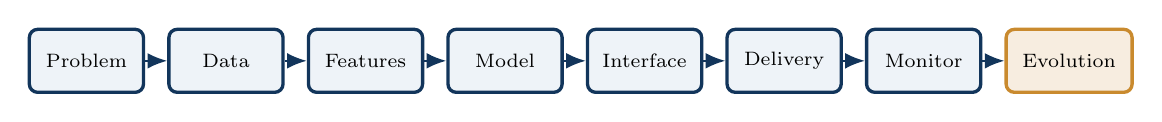
\begin{tikzpicture}[node distance=0.28cm]
  \node[flowbox, minimum width=1.45cm, minimum height=0.8cm] (problem) {\scriptsize Problem};
  \node[flowbox, minimum width=1.45cm, minimum height=0.8cm, right=of problem] (data) {\scriptsize Data};
  \node[flowbox, minimum width=1.45cm, minimum height=0.8cm, right=of data] (features) {\scriptsize Features};
  \node[flowbox, minimum width=1.45cm, minimum height=0.8cm, right=of features] (model) {\scriptsize Model};
  \node[flowbox, minimum width=1.45cm, minimum height=0.8cm, right=of model] (interface) {\scriptsize Interface};
  \node[flowbox, minimum width=1.45cm, minimum height=0.8cm, right=of interface] (delivery) {\scriptsize Delivery};
  \node[flowbox, minimum width=1.45cm, minimum height=0.8cm, right=of delivery] (monitor) {\scriptsize Monitor};
  \node[accentbox, minimum width=1.6cm, minimum height=0.8cm, right=of monitor] (evolution) {\scriptsize Evolution};
  \foreach \a/\b in {problem/data,data/features,features/model,model/interface,interface/delivery,delivery/monitor,monitor/evolution} {
    \draw[arrow] (\a) -- (\b);
  }
  \end{tikzpicture}

  \vspace{0.5em}
  \begin{block}{Today in the course}
  \textbf{Focus:} #1

  \textbf{Bridge:} #2
  \end{block}

  \begin{columns}[T]
  \column{0.48\textwidth}
  \begin{block}{Fraud case}
  {\footnotesize #3}
  \end{block}
  \column{0.48\textwidth}
  \begin{block}{Pasteurization case}
  {\footnotesize #4}
  \end{block}
  \end{columns}

  \vspace{0.3em}
  {\footnotesize \textbf{Course thread:} #5}
  \coursefooter
  \end{frame}
}

\newcommand{\classclosingframe}[4]{
  \begin{frame}{From This Class to the Next}
  \begin{block}{What stays with us}
  #1
  \end{block}

  \begin{columns}[T]
  \column{0.48\textwidth}
  \begin{block}{Project use}
  {\footnotesize #2}
  \end{block}
  \column{0.48\textwidth}
  \begin{block}{Next connection}
  {\footnotesize #3}
  \end{block}
  \end{columns}

  \vspace{0.3em}
  {\footnotesize \textbf{Course thread:} #4}
  \coursefooter
  \end{frame}
}

\tikzset{
  flowbox/.style={
    rounded corners=3pt,
    draw=courseblue,
    fill=courseice,
    very thick,
    minimum width=2.2cm,
    minimum height=0.9cm,
    align=center,
    font=\small
  },
  accentbox/.style={
    rounded corners=3pt,
    draw=coursegold,
    fill=coursegold!15,
    very thick,
    minimum width=2.2cm,
    minimum height=0.9cm,
    align=center,
    font=\small
  },
  arrow/.style={
    -{Latex[length=2.5mm,width=2mm]},
    thick,
    draw=courseblue
  }
}


\title{Class 12: Guided Lab --- EDA Practice}
\author{\coursename}
\date{}

\begin{document}

\frame{\titlepage \coursefooter}

\begin{frame}{Agenda}
\begin{itemize}
\item Lab format: hands-on, not lecture --- you drive, we circulate.
\item Reusing the Class 10 EDA workflow on a dataset you have not seen yet.
\item Three dataset options, same checklist, different data.
\item What a finished lab notebook should contain.
\end{itemize}
\coursefooter
\end{frame}

\begin{frame}{Learning goals}
\learninggoals{
\begin{itemize}
\item Apply the Class 10 EDA workflow to a new dataset without step-by-step guidance.
\item Load a scikit-learn bundled dataset into a pandas DataFrame from scratch.
\item Produce missing-value checks, summary statistics, and at least two plots unaided.
\item State one hypothesis about feature separability, backed by what you plotted.
\end{itemize}
}
\coursefooter
\end{frame}

\coursecontextframe
{Guided practice: the same EDA workflow, a dataset you pick yourself.}
{Class 10 walked through EDA on iris step by step; today the steps are the same, but you choose the dataset and drive.}
{This is the same discipline the fraud case needed before any model was trusted: load, check, visualize, hypothesize.}
{It is also what the pasteurization case needs the first time a new batch of synthetic sensor data is generated.}
{The workflow, not the dataset, is the thing you are practicing today.}

\begin{frame}{How this lab is structured}
\begin{enumerate}
\item Pick one dataset: Wine, Breast Cancer, or Digits (all built into scikit-learn).
\item Load it into a pandas DataFrame.
\item Run the same checklist as `Class2\_EDA.ipynb`: missingness, descriptive statistics, distributions, correlations.
\item Write one or two hypotheses about which features separate the classes best.
\end{enumerate}
\repoactivity{
`notebooks/Class2\_EDA\_Exercise.ipynb` is this lab, already in the repository --- open it and work directly inside it.
}
\coursefooter
\end{frame}

\begin{frame}[fragile]{Starter code}
\begin{lstlisting}[style=coursepython]
from sklearn.datasets import load_wine
import pandas as pd

wine = load_wine()
df_wine = pd.DataFrame(wine.data, columns=wine.feature_names)
df_wine['target'] = wine.target

print(df_wine.head())
print(df_wine['target'].value_counts())
\end{lstlisting}
\begin{itemize}
\item From `Class2\_EDA\_Exercise.ipynb`: the same pattern applies to \texttt{load\_breast\_cancer} and \texttt{load\_digits}, just change the loader.
\item Everything after this point is exactly Class 9 and Class 10 material, applied to unfamiliar columns.
\end{itemize}
\coursefooter
\end{frame}

\begin{frame}{Option A: Wine}
\begin{itemize}
\item 178 samples, 13 chemical-property features, 3 classes.
\item Suggested angle: how do the three wine classes differ in alcohol content, phenols, and color intensity?
\end{itemize}
\coursefooter
\end{frame}

\begin{frame}{Option B: Breast Cancer}
\begin{itemize}
\item 569 samples, 30 features describing cell-nuclei characteristics, 2 classes.
\item Suggested angle: which features look most discriminative between malignant and benign cases?
\end{itemize}
\coursefooter
\end{frame}

\begin{frame}{Option C: Digits}
\begin{itemize}
\item 1{,}797 samples, 8$\times$8 pixel images of handwritten digits, 10 classes.
\item Suggested angle: what do pixel-intensity correlations and per-digit distributions look like?
\end{itemize}
\coursefooter
\end{frame}

\begin{frame}{The checklist, whichever dataset you picked}
\begin{tabularx}{\textwidth}{>{\bfseries}l X}
Step & What to produce \\
\toprule
Missingness & \texttt{isnull().sum()} per column. \\
Descriptive stats & \texttt{.describe()}, and \texttt{.value\_counts()} on the target. \\
Distributions & At least one histogram or boxplot per class. \\
Correlations & A correlation heatmap across numeric features. \\
Pairwise view & A pairplot, if the feature count makes it readable. \\
\bottomrule
\end{tabularx}
\coursefooter
\end{frame}

\begin{frame}{What a finished lab notebook should contain}
\begin{itemize}
\item Every checklist item above, run and visible in the notebook output.
\item One or two written hypotheses about which features separate the classes, in your own words.
\item Nothing about modeling or metrics yet --- that is deliberately still ahead of us in the Data-Driven block.
\end{itemize}
\coursefooter
\end{frame}

\begin{frame}{Discussion prompt}
\begin{block}{Question}
Compare notes with someone who picked a different dataset. Did the same checklist surface different \emph{kinds} of insight on Wine versus Digits?
\end{block}
\begin{itemize}
\item Makes the point that the workflow generalizes even when the data semantics are completely different.
\end{itemize}
\coursefooter
\end{frame}

\begin{frame}{Papers and materials}
\readinglist{
\href{https://scikit-learn.org/stable/}{scikit-learn documentation};\
\href{https://pandas.pydata.org/docs/}{pandas documentation};\
\href{https://www.tandfonline.com/doi/abs/10.1080/01621459.1977.10480935}{Tukey (1977), Exploratory Data Analysis}.
}
\coursefooter
\end{frame}

\classclosingframe
{\begin{itemize}
\item The EDA workflow from Class 10 transfers to any tabular dataset with minimal changes.
\item Running the checklist unaided, on data you have not seen before, is the real test of whether it was learned.
\item This closes the Python block: twelve classes from ``what is Python'' to a working, repeatable analysis habit.
\end{itemize}}
{Your own course project's first deliverable should look exactly like this lab's checklist, applied to your project's dataset.}
{The Data-Driven block picks up from here with PCA, feature engineering, modeling, and evaluation --- the theory behind the choices this lab only hinted at.}
{Twelve classes of programming instrumentation now support everything the rest of the course will ask of that data.}

\end{document}
